\documentclass[12pt, a4paper,twoside]{tesi_upf}


%CODIFICACI�
\usepackage[latin1]{inputenc}


%IDIOMES
\usepackage[catalan,english]{babel}

%NOM�S PER A OBTENIR INDICACI� DEL MARC EN MIDA A4
\usepackage[cam,a4,center,frame]{crop}

%PER A INCLOURE GR�FICS I EL LOGO DE LA UPF
\usepackage{graphicx}
\usepackage{caption}
\usepackage{acronym}

%FONTS TIMES O GARAMOND, 
\usepackage{times}
%\usepackage{garamond}

%SENSE HEADINGS: NO MODIFICAR
\pagestyle{plain}

%PER A L'�NDEX DE MAT�RIES
\usepackage{makeidx}
\makeindex

%ESTIL DE BIBLIOGRAFIA
\bibliographystyle{apalike}


%AQUEST DOCUMENT �S EN CATAL�
\selectlanguage{english}

%EN COMPTES DE �NDEX, LA TAULA DE CONTINGUTS ES TITULA SUMARI
\addto\captionscatalan
  {\renewcommand{\contentsname}{\Large \sffamily Sumari}}


%AFEGIU EN AQUESTA PART LES VOSTRES DADES
\title{El t�tol de la tesi: Obligatori}
\subtitle{El subt�tol de la tesi: Opcional}
\author{Autor: Obligatori}
\thyear{L'any de la tesi: Obligatori}
\department{Departament: Obligatori}
\supervisor{Director: Obligatori}


\begin{document}


\frontmatter

\maketitle

\cleardoublepage


%%%%%% Dedicat�ria; si no es vol posar, comenteu fins a final de dedicat�ria

\noindent Escriviu aqu� la vostra dedicat�ria

\cleardoublepage

%%%%%% Final de dedicat�ria


%%%%%% Agra�ments; si no es vol posar, comenteu fins a final de agra�ments
\noindent {\Large \sffamily Agra�ments} Agraeixo....

\cleardoublepage

%%%%%% Final dels agra�ments

%ABSTRACT EN DOS IDIOMES. COM A M�NIM CATAL�. SI L'ALTRE �S EN CASTELLA CANVIEU EL QUE POSA ABSTRACT
\selectlanguage{english}
\section*{\Large \sffamily Abstract}
This is the abstract of the thesis in English.  Please, use less
than 150 words.

\selectlanguage{catalan}
\vspace*{\fill}
\section*{\Large \sffamily  Resum}
Vet aqu� el resum de la tesi en catal�.  Si us plau, utilitzeu
menys de 150 paraules.
\vspace*{\fill}

\selectlanguage{english}
\cleardoublepage
%FIN DE ABSTRACTE

%PREFACI OPCIONAL. SI NO ES VOL, COMENTEU FINS EL FINAL DE PREFACI
{\bf Prefaci}

\cleardoublepage
%FINAL DE PREFACI


%TAULA DE CONTINGUTS: OBLIGAT�RIA
\tableofcontents

%INDEX DE FIGURES; NOM�S ES POSA SI HI HA FIGURES
\listoffigures
%Fa que aparegui al sumari
\addcontentsline{toc}{chapter}{List of figures}

%INDEX DE TAULES; NOM�S ES POSA SI HI HA TAULES
\listoftables
%Fa que aparegui al sumari
\addcontentsline{toc}{chapter}{List of tables}

\cleardoublepage
\thispagestyle{empty}
\addcontentsline{toc}{chapter}{List of Abbreviations}
\vspace*{1.95cm} \hspace*{-0.155cm} %,88
\textbf{{\huge \sffamily List of Abbreviations}\\}
\vspace*{0.5cm}         
\begin{acronym}

\acro{WMN}{Wireless Mesh Networks}
\acro{AP}{Access Point}
\acro{BSS}{Basic Service Set}
\acro{MANET}{Mobile Ad-Hoc Network}
\acro{GSF}{Gracia Sense fils}
\acro{QMP}{Quick Mesh Project}

\end{acronym}

%COMEN�A EL TEXT
\mainmatter
\chapter{Introduction}
TODO
\chapter{State of the Art}

This project consists on studying how are, currently, being build  the open mesh networks in cities and what mechanisms we have to contribute or improve them. There are many different ways to improve this networks, namely, we can use different hardware, different software, build applications which run over them, etc.

First of all, we will analyze how these networks are, and how are they operating to have a better idea of what we want to improve.

\section{Mesh and MANET networks}

\subsection{Definition and properties}

When we talk about mesh networks, we refer to networks where all the participant are also routers. If we had to set a single definition the following can be a good one:
\\[10pt]
"\textit{A Mesh network is one where all nodes (participants) are routers, meaning that all the nodes accept and forward packets from other nodes according to the routing rules.}" \cite{paupfc}
\\[12pt] 
%Acronimo para a�adir
More specifically, we want to talk about \ac{WMN} which may refer also to the users of the network, and can be defined as follows:
\\[10pt]
"\textit{Wireless mesh networks often consist of mesh clients, mesh routers and gateways. The mesh clients are often laptops, cell phones and other wireless devices while the mesh routers forward traffic to and from the gateways which may but need not connect to the Internet.}" \cite{huynhsimulation}
\\[12pt]

To summarize, we have that mesh networks are basically networks which are not defined by the topology (physical layer) or the kind of links between two nodes (link layer). They are defined by the way the nodes operate among them, there are not master/slave or node/supernode distinctions and so, all the nodes have a similar function. In addition, the clients (end users) do not notice any difference (between mesh or other kind of networks) when they connect to the mesh, they are totally transparent for them. 
\\[12pt]

As mentioned above, there are only two different kind of nodes: mesh routers and mesh gateways. They operate in exactly the same way when they have to route packets within the network, the only difference is that the gateways may be connected to a wider network, namely, the Internet and they can route packets to this other network. So, mesh routers just route packets inside the mesh while mesh gateways can also route packets to the outside. 
\\[12pt]

	\noindent%
\begin{minipage}{\linewidth}
\vspace{10 mm}
\makebox[\linewidth]{%
  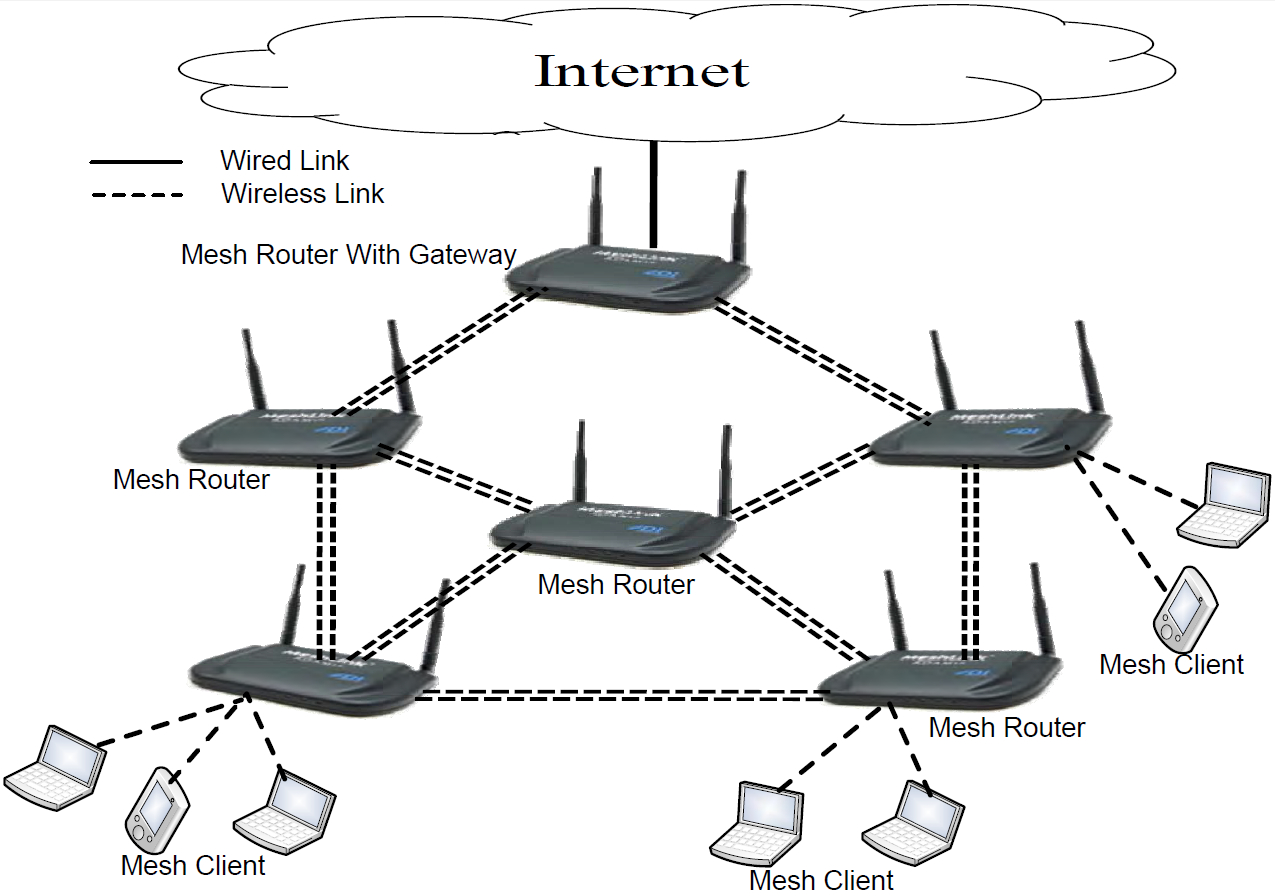
\includegraphics[width=0.8 \linewidth]{Images/wmn11.jpg}}
\captionof{figure}{Wireless Mesh Network Example}% only if needed
\caption*{http://www.intechopen.com/source/html/37888/media/wmn11.jpg}
\label{city}
\end{minipage}
\nocite{WMNs}
\clearpage

Then, we can say that WMN are a subtype of mesh networks. They have all the properties of these networks with the only difference that all the nodes are connected wirelessly. 

\subsection{Operating modes}
\nocite{qmpPresentation}

Mesh networks can operate in two different modes: Infrastructure mode and Ad-Hoc mode.

\begin{itemize}
	\item \textbf{Infrastructure Mode: }In this mode we have a central point named \ac{AP} that creates a \ac{BSS} zone in which all the packets have to go through the AP. This zone is identified by the MAC address of the AP, which is called BSSID in this context. Furthermore, we can say that a master/slave model is followed in infrastructure mode.
	
		\noindent%
\begin{minipage}{\linewidth}
\vspace{10 mm}
\makebox[\linewidth]{%
  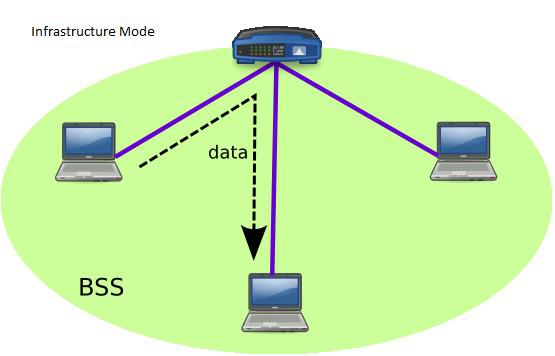
\includegraphics[width=0.8 \linewidth]{Images/InfMode.png}}
\captionof{figure}{Infrastructure Mode BSS}% only if needed
\caption*{\cite{qmpPresentation}}
\label{Infrastructure}
\end{minipage}

\clearpage
	\item \textbf{Ad-Hoc Mode: }In Ad-Hoc mode, all the participants play the same role. Therefore, every single node connects with all the nodes it can, and so the central point idea disappears. To identify which participants are in the same network we just need to find those who have the same BSSID. At this point, all the machines directly connected can exchange information but, a layer 3 routing protocol is required to allow the communication between nodes which are not connected directly. 
	
	\noindent%
\begin{minipage}{\linewidth}
\vspace{10 mm}
\makebox[\linewidth]{%
  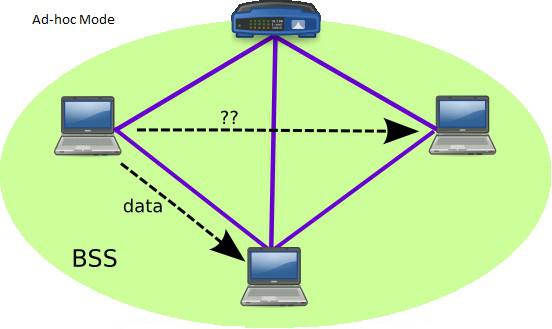
\includegraphics[width=0.8 \linewidth]{Images/AdhocMode.png}}
\captionof{figure}{Ad-Hoc Mode BSS}% only if needed
\caption*{\cite{qmpPresentation}}
\label{Ad-hoc}
\end{minipage}
\end{itemize}

\subsection{MANET Networks}

\ac{MANET} is a subtype of a mesh network. That is to say, when we have a mesh network which uses a wireless system to interconnect the nodes and is built in Ad-hoc mode, we talk about \ac{MANET}. Another way to define it can be: A \ac{MANET} network is a \ac{WMN} which operates in Ad-Hoc mode. 
\\[12pt]

Usually, when we talk about \ac{MANET} we are also referring to networks which have a self-configuring property. This property relies on the fact that the routers within the network are free-to-move anytime and to anywhere. A good definition could be this:
\\[12pt]

"\textit{A Mobile Ad hoc NETwork (MANET) is a kind of wireless ad-hoc network, and is a self-configuring network of mobile routers (and associated hosts) connected by wireless links - the union of which forms an arbitrary topology.}"\cite{Manetdef}
\\[12pt]


\section{Open \ac{MANET} Networks in Barcelona}

Nowadays, in Barcelona (and in some other cities) some MANET networks are being deployed. We will study this case in particular because is the one we are more familiar with. In general terms, all the deployments work in the same manner and so, studying one single case can give us a general a idea of all of them.
\\[12pt]

Normally, all these deployments only differ in some points, these are the more relevant ones:

\begin{itemize}
	\item The funding scheme
	\item The kind of hardware
	\item The firmware used 
\end{itemize}


\subsection{Funding scheme in Barcelona's \ac{MANET} networks}

There are some examples of MANET networks successfully deployed in Barcelona:

\begin{itemize}
	\item Gr�cia
	\item Sants
	\item Poble Nou
	\item Sant Joan Desp�
\end{itemize}


All these networks have been deployed using the same funding scheme, promoted by the Guifi.net foundation, and is, somehow, based on crowd-funding. Basically, anyone can install a new node and join to the mesh. There is just one restriction: you have to have direct vision with, at least, another node in the network. If you achieve this requirement, you can buy and install the node yourself and you expand the network. So, this is crowd-funding because every person joining the network funds its own equipment, which has the only requirement of being compatible with the firmware used. Since many people has no experience on installing and configuring the nodes, and despite the fact that both the hardware and software are specially designed to allow non-technical people to use it without problems, the foundation provides technical support for those who do not achieve in the installation. 

\subsection{The Kind of hardware in Barcelona's \ac{MANET} networks}

Being that the users are the owners of the network and so, the people who buy the equipment, usually low-cost hardware is used. Low-cost does not mean, low-quality, in fact some of the hardware used have very high features and a very good performance. Normally, the hardware used is from Ubiquity Networks (NanoStation, Rocket, Bullet, etc.), but it is not strictly necessary. Actually, any hardware compatible with the linux distribution openWRT is accepted. 
\\[10pt]

There are more information about some of this devices in annex 2.

\subsection{The Firmware used in Barcelona's \ac{MANET} networks}

This is maybe the most important difference between all the deployments around the world. In most of them, there is a common point: all the firmwares are openWRT based, but they have some differences. Particularly, in Barcelona the first deployments used the \ac{GSF} firmware, developed since 2003 for the Gracia Sense Fils Wireless Community. Some year later, the firmware became outdated since the protocol versions where old and the configuration of the nodes was hard. Then, they decided to create a new firmware with bigger scope, they named it \ac{QMP} and is the one being used currently (some nodes have to be migrated to \ac{QMP} yet).







     



\chapter{Methodology}
TODO
\chapter{Contribution}

\chapter{Results}
TODO
\chapter{Conclusions}
TODO
\chapter{Future Work}
TODO






\bibliography{bibliography}



\backmatter
\printindex





\end{document}


%NUMERACI� DE LA P�GINA EXTERIOR EXCEPTE EN LA PRIMERA P�GINA DE CADA CAP�TOL
\usepackage{fancyhdr}
\pagestyle{fancy}
\fancyfoot{}
\fancyfoot[RO]{\thepage}
\fancyfoot[LE]{\thepage}


%MUTIPLES �NDEX
%En el pre�mbul
\usepackage{multind}
\makeindex{authors}
%Introducci� d'entrades la forma
\index{authors}{Einstein}
%Situaci� de l'�ndex
\printindex{authors}{Author index}
%Cal eliminar les comandes \usepakage{makeidx} \makeindex \printindex
%cal exacutar des de la l�nia de comandes makeindex authors